\documentclass[11pt]{article}

% ====================================================
% PACKAGES
% ====================================================
\usepackage[margin=1in, headheight=13.6pt]{geometry}
\usepackage[T1]{fontenc}
\usepackage{lmodern}
\usepackage{microtype}
\usepackage{setspace}
\usepackage{tcolorbox}
\usepackage{amsmath, amssymb, mathtools}
\usepackage{siunitx}
\usepackage{bm}

\usepackage{graphicx}
\usepackage{float}
\usepackage{subcaption}

\usepackage{enumitem}
\usepackage{booktabs}
\usepackage{longtable}
\usepackage{array}
\usepackage{multirow}

\usepackage{xcolor}
\usepackage{hyperref}

\usepackage{fancyhdr}
\usepackage{lastpage}

\usepackage{indentfirst}
\usepackage[justification=centering]{caption}
\usepackage{pdfpages}
\usepackage{listings}

\lstdefinestyle{pystyle}{
    language=Python,
    basicstyle=\ttfamily\small,
    keywordstyle=\color{blue!60!black}\bfseries,
    commentstyle=\color{green!40!black}\itshape,
    stringstyle=\color{orange!70!black},
    numbers=left,
    numberstyle=\tiny\color{gray},
    numbersep=6pt,
    breaklines=true,
    breakatwhitespace=false,
    showstringspaces=false,
    frame=single,
    rulecolor=\color{gray!50},
    tabsize=4
}
\lstset{style=pystyle}

\pagestyle{fancy}
\fancyhf{}
\lhead{\Assignment\ |\ \course}
\rhead{\Name\ |\ \today}
\cfoot{Page \thepage\ of~\pageref{LastPage}}

\hypersetup{
    colorlinks,
    linkcolor={red!50!black},
    citecolor={blue!50!black},
    urlcolor={blue!80!black}
}

\newcommand{\Name}{Arael Anaya}
\newcommand{\Assignment}{Homework 4}
\newcommand{\course}{Robot Mechanics}

% Boxed final-answer environment
\newtcolorbox{result}{
    colback=blue!3!white,
    colframe=blue!40!black,
    boxrule=0.6pt,
    arc=2pt,
    left=6pt, right=6pt, top=4pt, bottom=4pt
}

% Boxed problem-statement environment
\newtcolorbox{statement}{
    colback=gray!5!white,
    colframe=gray!50!black,
    boxrule=0.4pt,
    arc=2pt,
    left=6pt, right=6pt, top=4pt, bottom=4pt
}

% Visible placeholder for work not yet added
\newcommand{\workplaceholder}{%
    \par\vspace{4pt}\noindent\textcolor{gray!60}{\itshape [Work not yet added: paste solution here]}\par\vspace{4pt}%
}

% Boxed correction-note environment (flags a fix made to the original hand calc)
\newtcolorbox{fixnote}{
    colback=orange!5!white,
    colframe=orange!55!black,
    boxrule=0.5pt,
    arc=2pt,
    left=6pt, right=6pt, top=4pt, bottom=4pt,
    fontupper=\small
}

% Notation macros (matching course conventions)
\newcommand{\T}{\bm{T}}
\newcommand{\R}{\bm{R}}
\newcommand{\dvec}{\bm{d}}
\newcommand{\framen}[1]{\{#1\}}
\newcommand{\khat}{\widehat{\bm{k}}}
\newcommand{\wvec}{\bm{\omega}}
\newcommand{\xivec}{\bm{\xi}}
\newcommand{\vvec}{\bm{v}}
\newcommand{\Omvec}{\bm{\Omega}}
\newcommand{\Rotx}{\operatorname{Rot}_x}
\newcommand{\Roty}{\operatorname{Rot}_y}
\newcommand{\Rotz}{\operatorname{Rot}_z}
\newcommand{\atantwo}{\operatorname{atan2}}
\newcommand{\skewx}[1]{\left[#1\right]_{\times}}

\begin{document}

% ====================================================
% PROBLEM 1
% ====================================================
\section*{Problem 1}

\begin{statement}
Derive from the inverse twist problem equations (p.~34 of notes) the simplified forward and inverse
equations for the twist parameterization in the special case of parallel displacement $\dvec$ with the
rotation axis $\khat$.
\end{statement}

\workplaceholder

% ====================================================
% PROBLEM 2
% ====================================================
\newpage
\section*{Problem 2}

\begin{statement}
Sketch the zero-angle configuration from the following DH table.
\begin{center}
\begin{tabular}{c | c | c | c | c}
\hline
 Link & $a$ & $d$ & $\alpha$ & $\theta$\\  \hline
 $1$ & $1$   & $1$ & $\pi/2$  & $\star$ \\
 $2$ & $0.5$ & $1$ & $-\pi/2$ & $\star$ \\
 $3$ & $0$   & $0$ & $0$      & $\star$ \\
 $4$ & $1$   & $0$ & $\pi/2$  & $\star$ \\
 $5$ & $0$   & $0$ & $-\pi/2$ & $\star$ \\
 $6$ & $0$   & $0$ & $\pi/2$  & $\star$ \\ \hline
\end{tabular}
\end{center}
\end{statement}

\workplaceholder

% ====================================================
% PROBLEM 3
% ====================================================
\newpage
\section*{Problem 3}

\begin{statement}
Sketch the zero-angle configuration from the following DH table.
\begin{center}
\begin{tabular}{c | c | c | c | c}
\hline
 Link & $a$ & $d$      & $\alpha$ & $\theta$\\  \hline
 $1$ & $1$ & $\star$ & $\pi/2$ & $0$ \\
 $2$ & $1$ & $\star$ & $\pi/2$ & $\pi/2$ \\
 $3$ & $1$ & $\star$ & $0$     & $0$ \\ \hline
\end{tabular}
\end{center}
\end{statement}

\workplaceholder

% ====================================================
% PROBLEM 4
% ====================================================
\newpage
\section*{Problem 4}

\begin{statement}
For the manipulator of Problem 2:
\begin{enumerate}[label=(\alph*), leftmargin=1.6em, itemsep=2pt]
    \item What is the homogeneous transformation $\prescript{0}{}{\T}_6$ if all joint angles are $0$?
    \item What is the homogeneous transformation $\prescript{0}{}{\T}_6$ if all joint angles are $\pi/6$?
\end{enumerate}
\end{statement}

\subsection*{Part (a)}
\workplaceholder

\subsection*{Part (b)}
\workplaceholder

% ====================================================
% PROBLEM 5
% ====================================================
\newpage
\section*{Problem 5}

\begin{statement}
For the manipulator of Problem 3:
\begin{enumerate}[label=(\alph*), leftmargin=1.6em, itemsep=2pt]
    \item What is $\prescript{0}{}{\T}_3$ when $d_1 = 1$ and all other joints are $0$?
    \item What is $\prescript{0}{}{\T}_3$ when $d_2 = 1$ and all other joints are $0$?
    \item What is $\prescript{0}{}{\T}_3$ when $d_3 = 1$ and all other joints are $0$?
\end{enumerate}
\end{statement}

\subsection*{Part (a)}
\workplaceholder

\subsection*{Part (b)}
\workplaceholder

\subsection*{Part (c)}
\workplaceholder

% ====================================================
% PROBLEM 6
% ====================================================
\newpage
\section*{Problem 6}

\begin{statement}
Derive the DH parameters for the RRPR manipulator shown in the figure below.
\begin{center}
    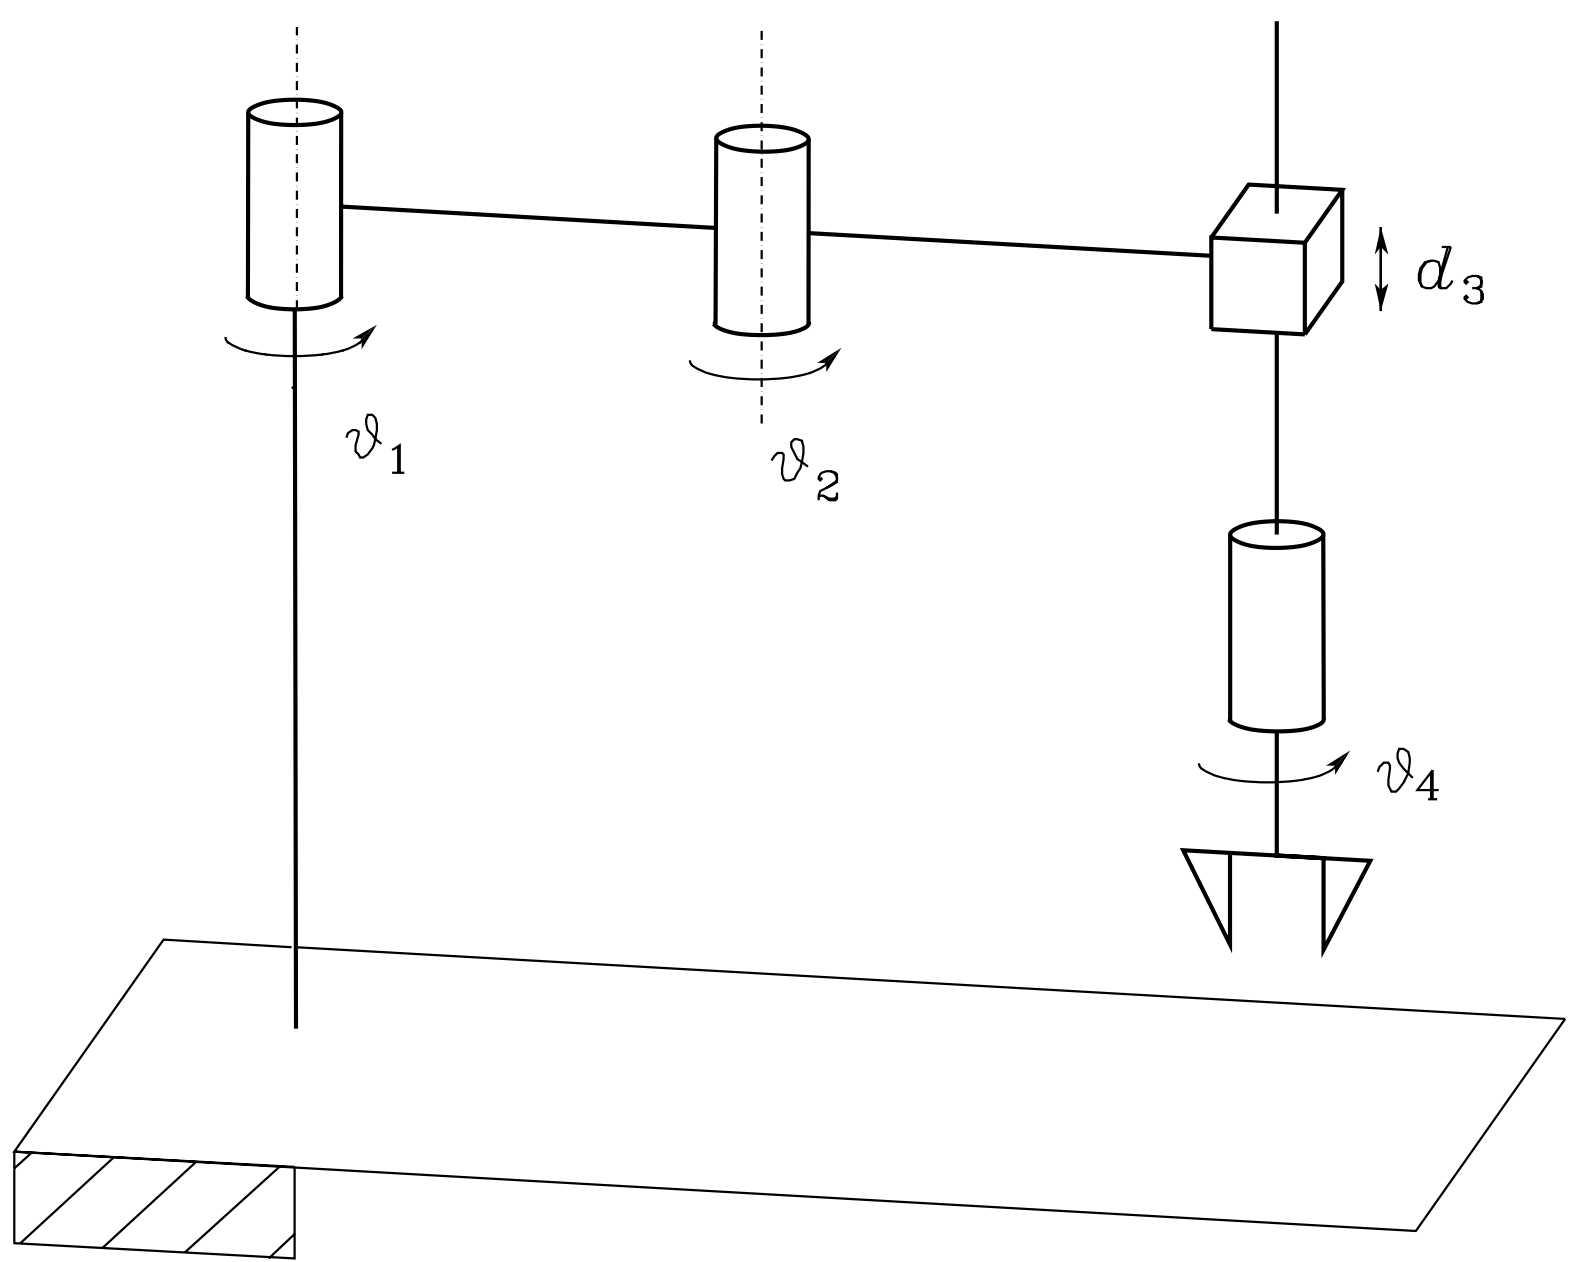
\includegraphics[width=.4\columnwidth]{Figures/SCARA_manipulator_siciliano_fig_2.36.png}
    \captionof{figure}{RRPR manipulator.}
\end{center}
\end{statement}

\workplaceholder

% ====================================================
% APPENDIX A: HAND CALCULATIONS
% ====================================================
\newpage
\section*{Appendix A: Hand Calculations}

\IfFileExists{../Homework_4_hand_calcs.pdf}{%
    \includepdf[pages=-, pagecommand={\thispagestyle{plain}}, scale=0.9]{../Homework_4_hand_calcs.pdf}%
}{%
    \noindent\textcolor{gray!60}{\itshape [Homework\_4\_hand\_calcs.pdf not yet added]}%
}

\end{document}
